% WR figure exported by sim_ui.py -- 2026-09-17 19:15:18
%
% Preamble (once, in your thesis):
%   \usepackage{pgfplots}
%   \pgfplotsset{compat=1.18}
%
% Use:
%   \begin{figure}[htbp]\centering
%     \input{wr_convergence}
%     \caption{...}\label{fig:...}
%   \end{figure}
%
% \input nests (unlike \include), so this works inside a chapter file the root
% already \includes. Pasting the body below inline works too -- the \definecolor
% lines may then be hoisted into the preamble and dropped from each figure.
%
% Series are thinned to ~2000 points each (min/max decimation, so spikes are
% preserved); edit _PGF_MAX_PTS in sim_ui.py for the full-resolution data.
%
% Run: coupling_mode=voltage-driven; precondition=on (optimized); interface_form=Thevenin (V source); use_t_floor=bare dt; interface_consistency=BDF-1/BE (naive); N_field_windows=50; N_xyce_samples=200; xyce_integration_method=Backward-Euler (maxord=1)

\definecolor{C0}{HTML}{1F77B4}
\definecolor{C1}{HTML}{FF7F0E}
\definecolor{C2}{HTML}{2CA02C}
\definecolor{C3}{HTML}{D62728}

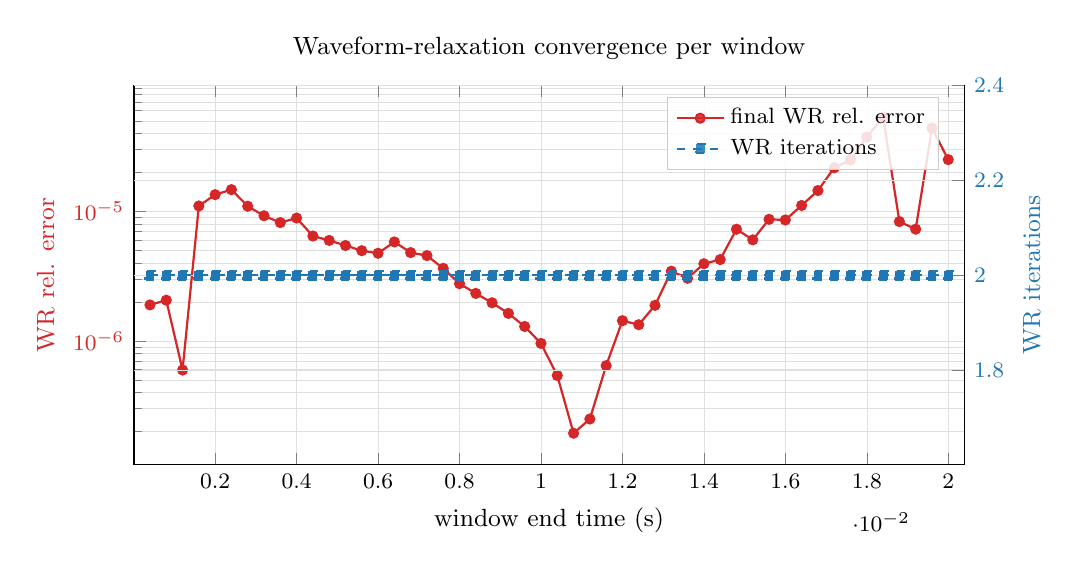
\begin{tikzpicture}
\begin{axis}[
  width=\linewidth,
  height=6.4cm,
  title={Waveform-relaxation convergence per window},
  xlabel={window end time (s)},
  ylabel={WR rel. error},
  grid=both,
  grid style={line width=.2pt, draw=gray!25},
  legend pos=north east,
  legend cell align=left,
  legend style={font=\footnotesize, fill=white, fill opacity=0.85, text opacity=1, draw=gray!40},
  tick label style={font=\footnotesize},
  label style={font=\small},
  title style={font=\small},
  scaled x ticks=true,
  xmin=8e-06,
  xmax=0.020392,
  ymode=log,
  axis y line*=left,
  ylabel style={color=C3},
  yticklabel style={color=C3}
]
  \addplot[color=C3, line width=0.8pt, mark=*, mark size=1.6pt] coordinates {
    (0.0004,1.896e-06) (0.0008,2.063e-06) (0.0012,5.954e-07) (0.0016,1.102e-05) (0.002,1.348e-05) (0.0024,1.474e-05)
    (0.0028,1.097e-05) (0.0032,9.254e-06) (0.0036,8.201e-06) (0.004,8.889e-06) (0.0044,6.456e-06) (0.0048,5.973e-06)
    (0.0052,5.455e-06) (0.0056,4.975e-06) (0.006,4.752e-06) (0.0064,5.814e-06) (0.0068,4.808e-06) (0.0072,4.557e-06)
    (0.0076,3.633e-06) (0.008,2.766e-06) (0.0084,2.327e-06) (0.0088,1.97e-06) (0.0092,1.631e-06) (0.0096,1.292e-06)
    (0.01,9.559e-07) (0.0104,5.403e-07) (0.0108,1.935e-07) (0.0112,2.491e-07) (0.0116,6.438e-07) (0.012,1.432e-06)
    (0.0124,1.333e-06) (0.0128,1.881e-06) (0.0132,3.453e-06) (0.0136,3.045e-06) (0.014,3.944e-06) (0.0144,4.246e-06)
    (0.0148,7.288e-06) (0.0152,6.032e-06) (0.0156,8.691e-06) (0.016,8.59e-06) (0.0164,1.112e-05) (0.0168,1.45e-05)
    (0.0172,2.175e-05) (0.0176,2.503e-05) (0.018,3.749e-05) (0.0184,5.36e-05) (0.0188,8.349e-06) (0.0192,7.295e-06)
    (0.0196,4.405e-05) (0.02,2.513e-05)
  };
\end{axis}
\begin{axis}[
  width=\linewidth,
  height=6.4cm,
  title={},
  xlabel={},
  ylabel={WR iterations},
  grid=both,
  grid style={line width=.2pt, draw=gray!25},
  legend pos=north east,
  legend cell align=left,
  legend style={font=\footnotesize, fill=white, fill opacity=0.85, text opacity=1, draw=gray!40},
  tick label style={font=\footnotesize},
  label style={font=\small},
  title style={font=\small},
  scaled x ticks=true,
  xmin=8e-06,
  xmax=0.020392,
  axis y line*=right,
  axis x line=none,
  ylabel style={color=C0},
  yticklabel style={color=C0}
]
  \addlegendimage{color=C3, line width=0.8pt, mark=*, mark size=1.6pt}
  \addlegendentry{final WR rel. error}
  \addplot[color=C0, line width=0.8pt, dashed, mark=square*, mark size=1.6pt] coordinates {
    (0.0004,2) (0.0008,2) (0.0012,2) (0.0016,2) (0.002,2) (0.0024,2)
    (0.0028,2) (0.0032,2) (0.0036,2) (0.004,2) (0.0044,2) (0.0048,2)
    (0.0052,2) (0.0056,2) (0.006,2) (0.0064,2) (0.0068,2) (0.0072,2)
    (0.0076,2) (0.008,2) (0.0084,2) (0.0088,2) (0.0092,2) (0.0096,2)
    (0.01,2) (0.0104,2) (0.0108,2) (0.0112,2) (0.0116,2) (0.012,2)
    (0.0124,2) (0.0128,2) (0.0132,2) (0.0136,2) (0.014,2) (0.0144,2)
    (0.0148,2) (0.0152,2) (0.0156,2) (0.016,2) (0.0164,2) (0.0168,2)
    (0.0172,2) (0.0176,2) (0.018,2) (0.0184,2) (0.0188,2) (0.0192,2)
    (0.0196,2) (0.02,2)
  };
  \addlegendentry{WR iterations}
\end{axis}
\end{tikzpicture}
